% Don't touch this %%%%%%%%%%%%%%%%%%%%%%%%%%%%%%%%%%%%%%%%%%%
\documentclass[12pt]{article}
\usepackage{fullpage}
\usepackage[left=1in,top=1in,right=1in,bottom=1in,headheight=3ex,headsep=3ex]{geometry}
\usepackage{graphicx}
\usepackage{float}
\usepackage{array}


\newcommand{\blankline}{\quad\pagebreak[2]}
%%%%%%%%%%%%%%%%%%%%%%%%%%%%%%%%%%%%%%%%%%%%%%%%%%%%%%%%%%%%%%

% Modify Course title, instructor name, semester here %%%%%%%%

\title{PHY115: Homework 1}
\author{Spring 2021}
\date{}

%%%%%%%%%%%%%%%%%%%%%%%%%%%%%%%%%%%%%%%%%%%%%%%%%%%%%%%%%%%%%%

% Don't touch this %%%%%%%%%%%%%%%%%%%%%%%%%%%%%%%%%%%%%%%%%%%
\usepackage[sc]{mathpazo}
%\linespread{1.05} % Palatino needs more leading (space between lines)
\usepackage[T1]{fontenc}
\usepackage[mmddyyyy]{datetime}% http://ctan.org/pkg/datetime
\usepackage{advdate}% http://ctan.org/pkg/advdate
\newdateformat{syldate}{\twodigit{\THEMONTH}/\twodigit{\THEDAY}}
\newsavebox{\MONDAY}\savebox{\MONDAY}{Mon}% Mon
\newcommand{\week}[1]{%
%  \cleardate{mydate}% Clear date
% \newdate{mydate}{\the\day}{\the\month}{\the\year}% Store date
  \paragraph*{\kern-2ex\quad #1, \syldate{\today} - \AdvanceDate[4]\syldate{\today}:}% Set heading  \quad #1
%  \setbox1=\hbox{\shortdayofweekname{\getdateday{mydate}}{\getdatemonth{mydate}}{\getdateyear{mydate}}}%
  \ifdim\wd1=\wd\MONDAY
    \AdvanceDate[7]
  \else
    \AdvanceDate[7]
  \fi%
}
%\usepackage{setspace}
\usepackage{multicol}
%\usepackage{indentfirst}
\usepackage{fancyhdr,lastpage}
\usepackage{url}
\pagestyle{fancy}
\usepackage{hyperref}
\usepackage{lastpage}
\usepackage{amsmath}
\usepackage{layout}

\lhead{}
\chead{}
%%%%%%%%%%%%%%%%%%%%%%%%%%%%%%%%%%%%%%%%%%%%%%%%%%%%%%%%%%%%%%

% Modify header here %%%%%%%%%%%%%%%%%%%%%%%%%%%%%%%%%%%%%%%%%
%\rhead{\footnotesize Text in header}

%%%%%%%%%%%%%%%%%%%%%%%%%%%%%%%%%%%%%%%%%%%%%%%%%%%%%%%%%%%%%%
% Don't touch this %%%%%%%%%%%%%%%%%%%%%%%%%%%%%%%%%%%%%%%%%%%
\lfoot{}
\cfoot{\small \thepage/\pageref*{LastPage}}
\rfoot{}

\usepackage{array, xcolor}
\usepackage{color,hyperref}
\definecolor{clemsonorange}{HTML}{EA6A20}
\hypersetup{colorlinks,breaklinks,linkcolor=clemsonorange,urlcolor=clemsonorange,anchorcolor=clemsonorange,citecolor=black}

\begin{document}

\maketitle

%\blankline

%\begin{tabular*}{.93\textwidth}{@{\extracolsep{\fill}}lr}

%%%%%%%%%%%%%%%%%%%%%%%%%%%%%%%%%%%%%%%%%%%%%%%%%%%%%%%%%%%%%%


\begin{center}
 Deadline: March 11th    
\end{center}
\hrule



% First Section %%%%%%%%%%%%%%%%%%%%%%%%%%%%%%%%%%%%%%%%%%%%

\section{Discusion Questions: 30 p}

\begin{enumerate}
  \item A crate of books rests on a level floor. To move it along the
  floor at a constant velocity, why do you exert a smaller force if you
  pull it at an angle $\theta$ above the horizontal than if you push it at the
  same angle below the horizontal?
  \item In a world without friction, which of the following activities
  could you do (or not do)? Explain your reasoning. (a) drive around
  an unbanked highway curve; (b) jump into the air; (c) start walking
  on a horizontal sidewalk; (d) climb a vertical ladder; (e) change
  lanes on the freeway.
  \item You are pushing a large crate from the back of a freight elevator
  to the front as the elevator is moving to the next floor. In
  which situation is the force you must apply to move the crate the
  smallest and in which is it the largest: when the elevator is accelerating
  upward, when it is accelerating downward, or when it is traveling
  at constant speed? Explain.
\end{enumerate}

\section*{Exercise 1: 30 p }
Consider an incline plane as the one shown in figure \ref{fig}, the box is at equilibrium and the friction coefficient
is $\mu_s$

\begin{itemize}
  \item If the inclination is $\alpha$ and the mass $m$, calculate the normal and the friction forces.
  \item Obtain an expression for $\mu_s$ in terms of $\alpha$.
  \item At what angle will the box start sliding?
\end{itemize}




\begin{figure}[h!]
  \begin{center}
    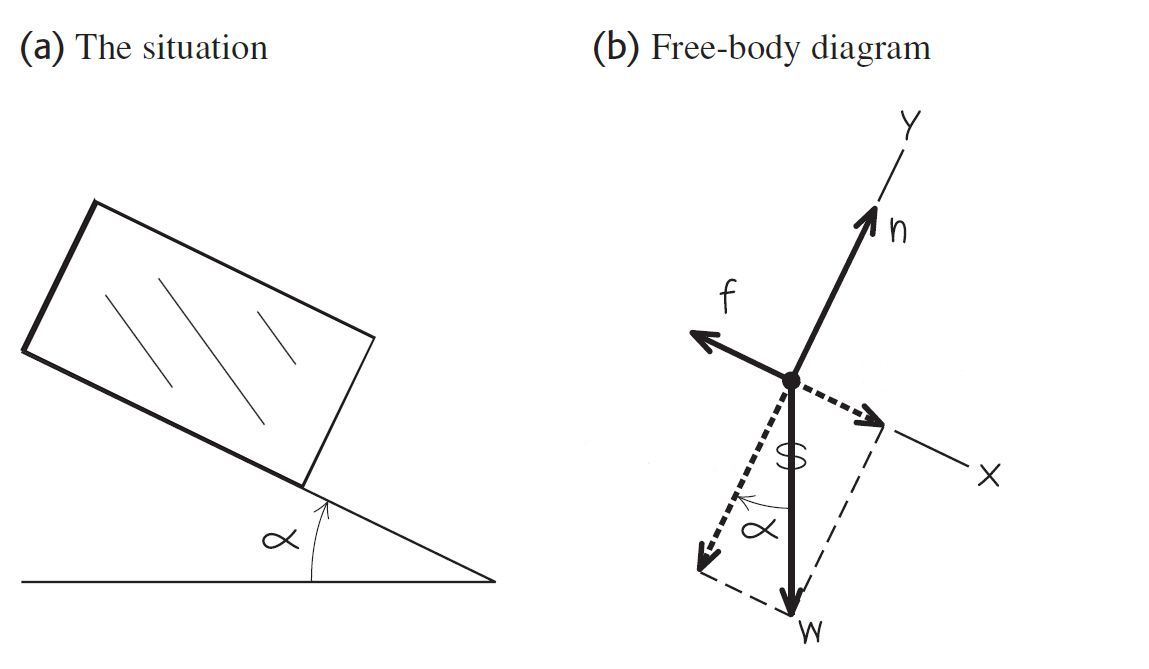
\includegraphics[width=0.65\textwidth]{images/2.jpg}
\label{fig}
  \end{center}
 
\end{figure}



\section*{Exercise 2: 40 p}

Let us simulate a falling  marble in different fluids.



\begin{itemize}
  \item Consider that the sphere mass is $1~kg$, and the radius is 1 m.
  \item The drag coefficient $k$ for different fluid is shown in the table. 
\end{itemize}


\begin{center}
  \begin{tabular}{c | c  }
    \hline
\hline
    Fluid & $k$ ($kg/s$) \\
    \hline
    \hline
   Air & $4\time 10^{-4}$  \\ 
   Water & $2\time 10^{-2}$   \\  
   Olive Oil & $1.5$      
  \end{tabular}
  \end{center}



  \begin{enumerate}
    \item Calculate the terminal velocity $v_t$ for each one of the fluids.
    \item Simulate the motion of the marble for each one of the fluids in 3ds Max. The expression for the motion in $z$ is,
  \end{enumerate}

\begin{equation}
  z=v_t\left[ t-\frac{m}{k}(1-e^{-(\frac{k}{m})t})  \right]
\end{equation}


3. In which fluid the marble reaches the terminal velocity first?

\vspace{4mm}

4.  What happens if you increase the mass?

\vspace{8mm}

\textbf{Hint: $e^{N}$ in 3ds Max is $exp(N)$ }




\section*{Extra credit: 20 p}

Model in 3ds Max a box of Aluminum sliding in a plane of steel with an inclination of $30$ degrees (neglect the air resistance).



\end{document}


